\chapter{Channel Coding}

\section{Noisy Channels}

\subsection{The Big Picture}
\begin{itemize}
    \item Previously, we explored source codes under ideal, noiseless conditions.
    \item However, this assumption is often unrealistic in practical communication settings.
    \item This lecture introduces the concept of \textbf{noisy channels}, where communication occurs in the presence of noise, affecting both transmission and reception.
\end{itemize}

\subsection{Discrete Memoryless Channel (DMC)}

\defb{Discrete Memoryless Channel}{
    A \textbf{discrete memoryless channel (DMC)} consists of:
    \begin{itemize}
        \item \textbf{Input alphabet} \( X \)
        \item \textbf{Output alphabet} \( Y \)
        \item \textbf{Conditional probability distribution} \( p(y|x) \), which represents the probability of receiving output \( y \) given input \( x \).
    \end{itemize}
    For longer messages, we consider the \textbf{extended channel} \( p(y^n|x^n) = \prod_{i=1}^{n} p(y_i|x_i) \), where \( n \) independent transmissions occur in parallel.
}

\subsection{Binary Symmetric Channel (BSC)}
\begin{marginfigure}
    \centering
    \begin{tikzpicture}[->, >=stealth, node distance=1cm]
        % Nodes for input and output states, positioned relatively
        \node (x0) {\( x = 0 \)};
        \node (x1) [below=of x0] {\( x = 1 \)};
        \node (y0) [right=of x0] {\( y = 0 \)};
        \node (y1) [right=of x1] {\( y = 1 \)};

        % Arrows for correct transmission with labels
        \draw[->] (x0) -- (y0) node[midway, above] {};
        \draw[->] (x1) -- (y1) node[midway, above] {};

        % Arrows for flip (error) with labels
        \draw[->] (x0) -- (y1) node[midway, right] {};
        \draw[->] (x1) -- (y0) node[midway, left] {};
    \end{tikzpicture}
    \caption{Binary Symmetric Channel}
\end{marginfigure}

\begin{itemize}
    \item A Binary Symmetric Channel (BSC) is a specific type of DMC with binary input and output alphabets, where each transmitted bit has a probability \( f \) of being flipped.
    \item Transmission probabilities:
          \begin{align*}
              P(y = 0 | x = 0) & = 1 - f, & P(y = 1 | x = 0) & = f,     \\
              P(y = 0 | x = 1) & = f,     & P(y = 1 | x = 1) & = 1 - f.
          \end{align*}
\end{itemize}

\ex{BSC of a Coin Flip}{
    \raggedright
    Consider a BSC with input distribution, \( p(X = 0) = p(X = 1) = 0.5 \), and a flip probability \( f \). \bigskip

    We recall the binary entropy function from Section \ref{sec:entropy_coin}, where \( H_2(f) = -f \log_2(f) - (1 - f) \log_2(1 - f) \) is the entropy of a Bernoulli distribution with parameter \( f \).

    \begin{itemize}
        \item We calculate the mutual information \( I(X; Y) \) between the input \( X \) and output \( Y \).
        \item Since conditional distribution \( p(Y | X) \) is Bernoulli and the channel is symmetric, meaning that
              \[ H(Y | X = 0) = H(Y | X = 1) = H_2(f) \]
        \item We then have
              \[
                  H(Y | X) = H_2(f)
              \]
        \item By symmetry, \( p(Y=0) = p(Y=1) = 0.5  \Rightarrow H(Y) = 1\), thus:
              \begin{align*}
                  I(X; Y) & = H(Y) - H(Y | X) \\ &= 1 - H_2(f)
              \end{align*}
    \end{itemize}
    Using these results, the mutual information \( I(X; Y) \) is:
    \[
        I(X; Y) = H(Y) - H(Y | X) = 1 - \big(-f \log_2(f) - (1 - f) \log_2(1 - f)\big)
    \]
}
\section{Channel Capacity}

\defb{Channel Capacity}{
    The capacity of a channel \(p(y|x)\) is defined as the maximum mutual information over all input distributions:
    \[
        C = \max_{p(x)} I(X; Y).
    \]
    The input distribution \(p^*(x)\) that achieves this maximum is known as the \textbf{capacity-achieving distribution}.
}

\sn{Open Questions}{
    \begin{itemize}
        \item In what sense is \(C\) a "capacity"?
        \item Can error-free communication be achieved at this capacity?
    \end{itemize}
}

\section*{Communication Without Errors: Noisy Typewriter}

\marginnote[8.5pt]{\sn{Connection to AEP}{
        The asymptotic equipartition property (AEP) suggests that all channels, for sufficiently large input blocks, behave analogously to the noisy typewriter.
    }}


\ex{Noisy Typewriter}{
    The input and output alphabets consist of 27 symbols (26 letters and a delimiter). Our input and output space are the same $|\mathcal{X}| = |\mathcal{Y}| = 27$. Typing a letter results in the letter or one of its two neighbours (we wrap around) with equal probability (\(1/3\)). So trying to type \textbf{A} could result in \textbf{A}, \textbf{B}, or \textbf{Z}, and trying to type \textbf{C} could result in \textbf{B}, \textbf{C}, or \textbf{D}.

    \bigskip

    Assuming a uniform input distribution:
    \begin{align*}
        H(Y)    & = \log 27 \, \text{bits},                \\
        H(Y|X)  & = \log 3 \, \text{bits},                 \\
        H(X|Y)  & = \log 3 \, \text{bits},                 \\
        I(X; Y) & = H(Y) - H(Y|X) = \log 9 \, \text{bits}.
    \end{align*}

    \begin{center}
        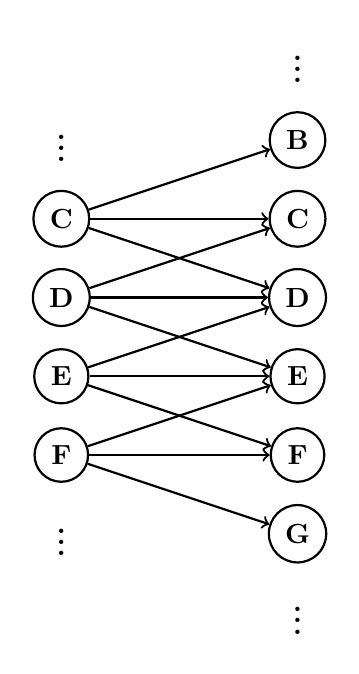
\begin{tikzpicture}[
                node distance=1.2cm and 1.2cm,
                every node/.style={circle, draw, minimum size=5mm, font=\bfseries},
                every path/.style={->, thick}
            ]

            % Define first column of nodes
            \node (C1) at (0,4) {C};
            \node (D1) at (0,3) {D};
            \node (E1) at (0,2) {E};
            \node (F1) at (0,1) {F};

            % Add vdots for the first column
            \node[draw=none, fill=none] (TopDots1) at (0,5) {\vdots};
            \node[draw=none, fill=none] (BottomDots1) at (0,0) {\vdots};

            % Define second column of nodes
            \node (B2) at (3,5) {B};
            \node (C2) at (3,4) {C};
            \node (D2) at (3,3) {D};
            \node (E2) at (3,2) {E};
            \node (F2) at (3,1) {F};
            \node (G2) at (3,0) {G};

            % Add vdots for the second column
            \node[draw=none, fill=none] (TopDots2) at (3,6) {\vdots};
            \node[draw=none, fill=none] (BottomDots2) at (3,-1) {\vdots};

            % Draw arrows from first column to second column
            % C1 -> B2, C2, D2
            \path (C1) edge (B2);
            \path (C1) edge (C2);
            \path (C1) edge (D2);

            % D1 -> C2, D2, E2
            \path (D1) edge (C2);
            \path (D1) edge (D2);
            \path (D1) edge (E2);

            % E1 -> D2, E2, F2
            \path (E1) edge (D2);
            \path (E1) edge (E2);
            \path (E1) edge (F2);

            % F1 -> E2, F2, G2
            \path (F1) edge (E2);
            \path (F1) edge (F2);
            \path (F1) edge (G2);

        \end{tikzpicture}
    \end{center}


}

\begin{figure}[h]
    \centering
    \includegraphics[width=\linewidth]{img/typewriter_unambiguous.png}
    \caption{The key is to use inputs with ambigious (or non-confusable) outputs.}
\end{figure}

In the noisy typewriter, we can achieve error-free communication by limiting the inputs to one of each 3 consecutive letters (e.g., \textbf{C}, \textbf{F}, \textbf{I}, \dots). Although this in practice reduces the messages we can send to only have 9 unique alphabets, we can receive them with absolute certainty.


\intuitb{Key Intuitions}{
    \begin{itemize}
        \item We achieve error-free communication by picking a non-confusable subset of inputs (i.e., inputs with disjoint output sets).
        \item In the same way as AEP makes all PDFs close to uniform, it also makes all channels close to the noisy typewriter.
    \end{itemize}


}

\defb{Channel Values}{
    \begin{itemize}
        \item Number of possible channel outputs: \(2^{nH(Y)}\).
        \item Number of confusable channel outputs for each input: \(2^{nH(Y|X)}\).
        \item Number of non-confusable input-output pairs:
              \[
                  \frac{\# \text{total outputs for all inputs}}{\# \text{confusable outputs per input}} = \frac{2^{nH(Y)}}{2^{nH(Y|X)}} = 2^{n(H(Y) - H(Y|X))} = 2^{nI(X;Y)}.
              \]
    \end{itemize}
}

\defb{Block code}{
    An \((n, K)\) block code \(\mathcal{S}\) is a set of \(2^K\) codewords, each of length \(n\). Mathematically:
    \[
        \{x^n(1), x^n(2), \dots, x^n(2^K)\}, \quad x^n(i) \in \mathcal{X}^n
    \]
}

\textbf{Intuitively:}
\begin{itemize}
    \item \(s \in \mathcal{S}\) are the source codewords, represented by a random variable \(S\) with distribution \(p(s) = 1/|\mathcal{S}| = 2^{-K}\). The corresponding channel input is \(x^n(s)\).
    \item \(n\) is the number of channel uses to send one word.
    \item \(K\) is the information (i.e., \textit{number of bits}) conveyed by one word.
    \item The \textit{rate} \(R = K / n\) is the number of bits conveyed per channel use.
\end{itemize}


\defb{Decoder}{
    A decoder is a mapping \(\mathcal{Y}^n \to \mathcal{S}\), denoted by \(\hat{s} = \text{Dec}(y^n)\), where \(y^n\) is the received sequence and \(\hat{s}\) is the estimated codeword. An additional output symbol \(s_0\) is often allowed to indicate a decoding failure.
}

\defb{Mean probability of block error}{
    The mean probability of block error, \(p_B\), quantifies the average likelihood that the decoded message \(\hat{s}\) differs from the transmitted codeword \(s\). It is given by:
    \[
        p_B = \sum_{s} p(s) p(\hat{s} \neq s \mid s)
    \]
}

\defb{Maximal probability of block error}{
    The maximal probability of block error, \(p_{B\text{M}}\), represents the worst-case likelihood of decoding failure over all possible transmitted codewords. It is defined as:
    \[
        p_{B\text{M}} = \max_{s} p(\hat{s} \neq s \mid s)
    \]
}

\defb{Probability of bit error}{
    The probability of bit error, \(p_b\), measures the likelihood that an individual bit within the transmitted message is incorrectly decoded. This applies to any of the \(K\) bits that comprise the codeword \(s\).
}

\section{Channel Coding Theorem}

\thm{Noisy Channel Coding}{
    Given a discrete memoryless channel:
    \begin{itemize}
        \item The channel capacity \(C\) has the following property: For any \(\epsilon > 0\) and \(R < C\), there exists a code of length \(n\) (for sufficiently large \(n\)) and a decoding algorithm such that the maximal block error probability satisfies \(p_{BM} < \epsilon\).
        \item If a probability of bit error \(p_b\) is acceptable, then rates up to \(R(p_b)\) are achievable, where
              \[
                  R(p_b) = \frac{C}{1 - H_2(p_b)}.
              \]
              Here, \(H_2(p_b)\) is the binary entropy function defined as:
              \[
                  H_2(p_b) = -p_b \log_2(p_b) - (1 - p_b) \log_2(1 - p_b).
              \]
        \item For any \(p_b\), rates greater than \(R(p_b)\) are not achievable.
    \end{itemize}
}

\intuitb{Code Space Partitioning}{
    The Channel Coding Theorem splits the space of codes into three regions:
    \begin{enumerate}
        \item A region where codes exist for all values of \(p_b\), including \(p_b = 0\).
        \item A region where faster codes exist but with some error (\(p_b > 0\)).
        \item A prohibited region where no codes are achievable.
    \end{enumerate}
}

\begin{center}
    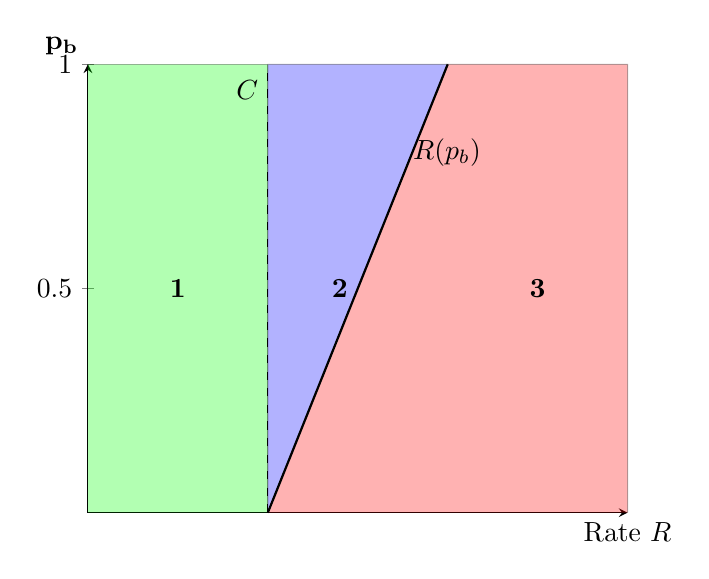
\begin{tikzpicture}
        \begin{axis}[
                axis x line=middle, axis y line=middle,
                xlabel={Rate \(R\)},
                ylabel={\(\mathbf{p_b}\)},
                xmin=0, xmax=1.5,
                ymin=0, ymax=1,
                xtick=\empty,
                ytick={0.5, 1},
                xlabel style={below},
                ylabel style={above left},
                clip=false
            ]

            % Region 1 (Green Rectangle)
            \addplot [fill=green, opacity=0.3] coordinates {
                    (0, 0)
                    (0.5, 0)
                    (0.5, 1)
                    (0, 1)
                    (0, 0)
                };

            % Region 2
            \addplot [fill=blue, opacity=0.3] coordinates {
                    (0.5, 0)
                    (0.5, 1)
                    (1, 1)
                    (0.5, 0)
                };

            % Region 3 (Red Region)
            \addplot [fill=red, opacity=0.3] coordinates {
                    (0.5, 0)
                    (1,1)
                    (1.5, 1)
                    (1.5, 0)
                    % (0.5, 1)
                };

            % R(pb) line
            \addplot [thick] coordinates {
                    (0.5, 0)
                    (1, 1)
                } node[pos=0.75, above right] {\(R(p_b)\)};

            % Capacity line
            \draw [dashed] (axis cs:0.5,0) -- (axis cs:0.5,1) node[pos=0.9, above left] {\(C\)};

            % Region Labels
            \node at (axis cs:0.25, 0.5) {\textbf{1}};
            \node at (axis cs:0.7, 0.5) {\textbf{2}};
            \node at (axis cs:1.25, 0.5) {\textbf{3}};

        \end{axis}
    \end{tikzpicture}
\end{center}

\section{Proving the First Statement of the Channel Coding Theorem}
\hl{Codes exist for all values of \(p_b\), including \(p_b = 0\).}

\defb{Typical Set Recap}{
    A \textbf{typical set}, denoted $\mathcal{A}_\epsilon^{(n)}$, is defined for sequences $x^n = (x_1, \dots, x_n)$ satisfying:

    \[
        \bigg| \frac{1}{n} \log p(x^n) - H(X) \bigg| \leq \epsilon,
    \]

    where $H(X)$ is the entropy of the source, and $\epsilon > 0$ is a small constant.

    \textbf{Key properties of the typical set:}
    \begin{enumerate}
        \item \textbf{Uniformity of Probabilities:} All sequences in $\mathcal{A}_\epsilon^{(n)}$ have approximately equal probabilities, $p(x^n) \approx 2^{-nH(X)}$. This arises because their average log-probabilities converge to $H(X)$ as $n \to \infty$.

        \item \textbf{High Probability of Occurrence:} The probability that a randomly chosen sequence belongs to the typical set satisfies:
              \[
                  P(x^n \in \mathcal{A}_\epsilon^{(n)}) > 1 - \epsilon,
              \]
              meaning that almost all observed sequences will lie within the typical set as $n$ increases.

        \item \textbf{Set Size Bounds:} The number of sequences in the typical set is tightly bounded as:
              \[
                  (1 - \epsilon) 2^{n(H(X) - \epsilon)} \leq |\mathcal{A}_\epsilon^{(n)}| \leq 2^{n(H(X) + \epsilon)}.
              \]
              This shows that the typical set captures nearly all the probability mass but represents a very small fraction of the $2^n$ possible sequences for large $n$.
    \end{enumerate}
}


\begin{figure}
    \includegraphics[width=\linewidth]{img/typical_set.png}
    \caption{Concentration of sequences in the typical set as $n$ increases.}
    \label{fig:typical_set}
\end{figure}

Figure \ref{fig:typical_set} illustrates the concentration of sequences as $n$ increases:
\begin{itemize}
    \item For $n = 10$, sequences are spread broadly across a range around $H(X)$, reflecting high variability for small $n$.
    \item For $n = 100$, the sequences concentrate more tightly within the interval $[H(X) - \epsilon, H(X) + \epsilon]$.
    \item For $n = 1000$, the concentration becomes even sharper, highlighting that as $n \to \infty$, almost all samples fall within the typical set and have equal likelihoods.
\end{itemize}
This is the asymptotic behaviour described by the Weak Law of Large Numbers, where the average properties of sequences converge to the entropy $H(X)$.

\defb{Jointly Typical Pairs}{
    Let $X, Y$ be joint random variables, and $X^n, Y^n$ be $n$ i.i.d. samples from $X, Y$. A pair $(x^n, y^n)$ belongs to the \textbf{jointly typical set}, $\mathcal{J}_\epsilon^{(n)}$, if the following conditions are satisfied:

    \begin{align}
        \bigg| \frac{1}{n} \log p(x^n) - H(X) \bigg|         & < \epsilon, \\
        \bigg| \frac{1}{n} \log p(y^n) - H(Y) \bigg|         & < \epsilon, \\
        \bigg| \frac{1}{n} \log p(x^n, y^n) - H(X, Y) \bigg| & < \epsilon.
    \end{align}

    \textbf{Intuition:}
    \begin{itemize}
        \item $x^n$ is typical with respect to $p(x^n)$ (marginal distribution of $X$),
        \item $y^n$ is typical with respect to $p(y^n)$ (marginal distribution of $Y$),
        \item and the pair $(x^n, y^n)$ is typical with respect to $p(x^n, y^n)$ (joint distribution of $X$ and $Y$).
    \end{itemize}
}

% \defb{Properties of Jointly Typical Pairs}{
Joint typicality has the following key properties:
\begin{enumerate}
    \item \textbf{Property 1:} If $(x^n, y^n) \in \mathcal{J}_\epsilon^{(n)}$, then:
    \[
    H(X, Y) - \epsilon \leq -\frac{1}{n} \log p(x^n, y^n) \leq H(X, Y) + \epsilon.
    \]
    \begin{itemize}
        \item \textit{In words:} All jointly typical events have almost the same probability.
        \item \textbf{Proof:} This follows directly from the definition of $\mathcal{J}_\epsilon^{(n)}$.
    \end{itemize}

    \item \textbf{Property 2:}
    \[
    \lim_{n \to \infty} \Pr\{ (x^n, y^n) \in \mathcal{J}_\epsilon^{(n)} \} = 1.
    \]
    \begin{itemize}
        \item \textit{In words:} Most samples are in the jointly typical set.
        \item \textbf{Proof:}
        \begin{itemize}
            \item Denote $\mathcal{A}(X)$, $\mathcal{A}(Y)$, and $\mathcal{A}(XY)$ as the typical sets for $X$, $Y$, and $(X, Y)$ respectively.
            \item For any sets $U, V$, we have $U \cap V = (U^c \cup V^c)^c$. Using the union bound:
            \[
            \Pr(U \cup V) \leq \Pr(U) + \Pr(V).
            \]
            \item Applying this to the complement of the jointly typical set:
            \[
            \Pr\{(x^n, y^n) \notin \mathcal{J}_\epsilon^{(n)} \} \leq \Pr\{x^n \notin \mathcal{A}(X)\} + \Pr\{y^n \notin \mathcal{A}(Y)\} + \Pr\{(x^n, y^n) \notin \mathcal{A}(XY)\}.
            \]
            \item As $n \to \infty$, all terms on the right-hand side vanish. Hence:
            \[
            \lim_{n \to \infty} \Pr\{(x^n, y^n) \in \mathcal{J}_\epsilon^{(n)}\} = 1.
            \]
        \end{itemize}
    \end{itemize}

    \item \textbf{Property 3:} The number of elements in $\mathcal{J}_\epsilon^{(n)}$ satisfies:
    \[
    |\mathcal{J}_\epsilon^{(n)}| \leq 2^{n(H(X, Y) + \epsilon)}.
    \]
    \begin{itemize}
        \item \textit{In words:} The number of items in $\mathcal{J}_\epsilon^{(n)}$ is upper-bounded by $2^{n(H(X, Y) + \epsilon)}$.
        \item \textbf{Proof:} Follows from the same reasoning used for the typical set $\mathcal{A}_\epsilon^{(n)}$.
    \end{itemize}

    \item \textbf{Property 4:} If $x^n$ and $\tilde{x}^n$ are independently sampled as $p(x^n)p(y^n)$, then:
    \[
    \Pr\{(x^n, y^n) \in \mathcal{J}_\epsilon^{(n)} \} \leq 2^{-n(I(X; Y) - 3\epsilon)},
    \]
    where $I(X; Y)$ is the mutual information between $X$ and $Y$.
    \begin{itemize}
        \item \textit{In words:} Independently sampled pairs are jointly typical with decreasing probability. The rate of decrease is governed by the mutual information.
        \item \textbf{Proof:}
        \begin{itemize}
            \item The probability of jointly typical pairs is given by:
            \[
            \Pr\{(x^n, y^n) \in \mathcal{J}_\epsilon^{(n)} \} = \sum_{(x^n, y^n) \in \mathcal{J}_\epsilon^{(n)}} p(x^n)p(y^n).
            \]
            \item Using the bounds on $|\mathcal{J}_\epsilon^{(n)}|$ and probabilities:
            \[
            \Pr\{(x^n, y^n) \in \mathcal{J}_\epsilon^{(n)} \} \leq 2^{n(H(X, Y) + \epsilon)} 2^{-n(H(X) - \epsilon)} 2^{-n(H(Y) - \epsilon)}.
            \]
            \item Simplifying:
            \[
            \Pr\{(x^n, y^n) \in \mathcal{J}_\epsilon^{(n)} \} \leq 2^{-n(I(X; Y) - 3\epsilon)}.
            \]
        \end{itemize}
    \end{itemize}
\end{enumerate}

\medskip

\textbf{Visualisation:}

\begin{center}
\includegraphics[width=\linewidth]{img/joint_dots.png}
\end{center}

\textit{Explanation of the figure:}
\begin{itemize}
    \item The horizontal span represents the typical set of $X$.
    \item The area covered by the dots represents the typical set of $(X, Y)$.
    \item Sampling from $p(x, y)$ corresponds to picking a dot at random.
    \item Sampling from $p(x)p(y)$ corresponds to picking a random point uniformly in the square.
    \item The ratio between the square's area and the number of dots is proportional to the mutual information $I(X; Y)$.
\end{itemize}

